\documentclass{ximera}  
\title{The Fourth Activity}  
\begin{document}  
\begin{abstract}  
A simple derivation problem.
\end{abstract}  
\maketitle    
  Display image.
\begin{image}  
  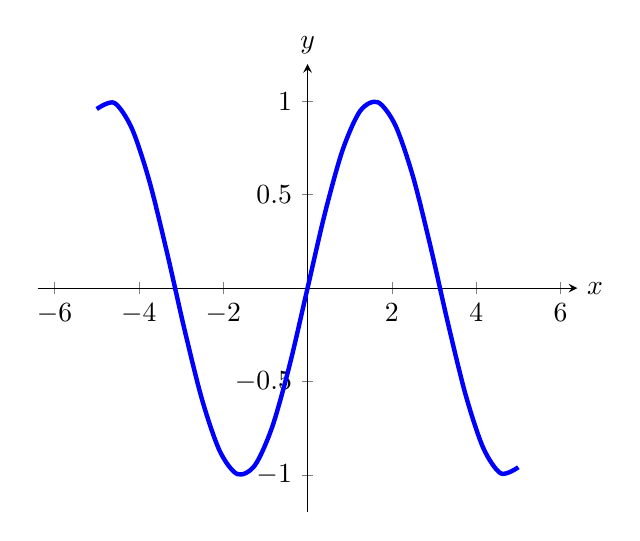
\begin{tikzpicture}  
    \begin{axis}[  
        xmin=-6.4,  
        xmax=6.4,  
        ymin=-1.2,  
        ymax=1.2,  
        axis lines=center,  
        xlabel=$x$,  
        ylabel=$y$,  
        every axis y label/.style={at=(current axis.above origin),anchor=south},  
        every axis x label/.style={at=(current axis.right of origin),anchor=west},  
      ]  
      \addplot [ultra thick, blue, smooth] {sin(deg(x))};  
    \end{axis}  
  \end{tikzpicture}  
\end{image} 

\end{document} 
